% This file was created by matlab2tikz.
%
%The latest updates can be retrieved from
%  http://www.mathworks.com/matlabcentral/fileexchange/22022-matlab2tikz-matlab2tikz
%where you can also make suggestions and rate matlab2tikz.
%
\definecolor{mycolor1}{rgb}{0.92900,0.69400,0.12500}%
\definecolor{mycolor2}{rgb}{0.85000,0.32500,0.09800}%
\definecolor{mycolor3}{rgb}{0.00000,0.44700,0.74100}%
%
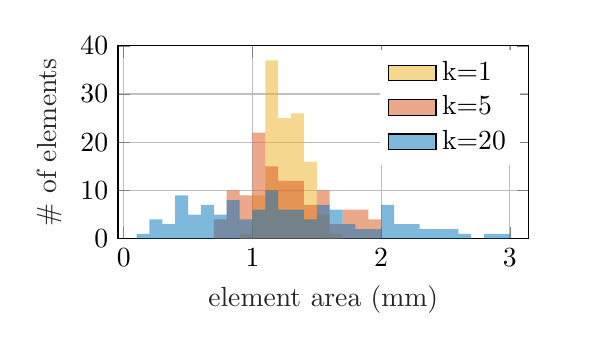
\begin{tikzpicture}

\begin{axis}[%
width=0.43\textwidth,
height=0.202\textwidth,
at={(0\textwidth,0\textwidth)},
scale only axis,
xmin=-0.0450000000000002,
xmax=3.145,
xlabel style={font=\color{white!15!black}},
xlabel={element area (mm)},
ymin=0,
ymax=40,
ylabel style={font=\color{white!15!black}},
ylabel={\# of elements},
axis background/.style={fill=white},
xmajorgrids,
ymajorgrids,
legend style={legend cell align=left, align=left, draw=none}
]
\addplot[ybar interval, fill=mycolor1, fill opacity=0.5, draw=none, area legend] table[row sep=crcr] {%
x	y\\
0.9	1\\
1	9\\
1.1	37\\
1.2	25\\
1.3	26\\
1.4	16\\
1.5	5\\
1.6	1\\
1.7	1\\
};
\addlegendentry{k=1}

\addplot[ybar interval, fill=mycolor2, fill opacity=0.5, draw=none, area legend] table[row sep=crcr] {%
x	y\\
0.7	4\\
0.8	10\\
0.9	9\\
1	22\\
1.1	15\\
1.2	12\\
1.3	12\\
1.4	7\\
1.5	10\\
1.6	3\\
1.7	6\\
1.8	6\\
1.9	4\\
2	4\\
};
\addlegendentry{k=5}

\addplot[ybar interval, fill=mycolor3, fill opacity=0.5, draw=none, area legend] table[row sep=crcr] {%
x	y\\
0.1	1\\
0.2	4\\
0.3	3\\
0.4	9\\
0.5	5\\
0.6	7\\
0.7	5\\
0.8	8\\
0.9	4\\
1	6\\
1.1	10\\
1.2	6\\
1.3	6\\
1.4	4\\
1.5	7\\
1.6	6\\
1.7	3\\
1.8	2\\
1.9	2\\
2	7\\
2.1	3\\
2.2	3\\
2.3	2\\
2.4	2\\
2.5	2\\
2.6	1\\
2.7	0\\
2.8	1\\
2.9	1\\
3	1\\
};
\addlegendentry{k=20}

\end{axis}

\begin{axis}[%
width=0.554\textwidth,
height=0.249\textwidth,
at={(-0.072\textwidth,-0.028\textwidth)},
scale only axis,
xmin=0,
xmax=1,
ymin=0,
ymax=1,
axis line style={draw=none},
ticks=none,
axis x line*=bottom,
axis y line*=left
]
\end{axis}
\end{tikzpicture}%